\chapter{EXPERIMENT ENVIRONMENT AND ARCHITECTURE}
\label{chap:experiment-implementation}

This chapter details the technical implementation of the experimental design defined in the previous chapter. To satisfy the requirement for scientific reproducibility, the entire experimental testbed—from the virtualization layer to the application deployment—was codified using Infrastructure as Code (IaC) principles.

Although cloud-managed Kubernetes services reflect prevalent industry practices, this research opted for a locally hosted, on-premise experimental testbed. This methodological decision is strictly grounded in the necessity for internal validity during the controlled experiment. Public cloud environments are inherently susceptible to multi-tenancy resource contention and the ``noisy neighbor'' effect, which introduce unpredictable fluctuations in CPU, memory, and network latency \cite{kuria_2024}.

Since the evaluation of the PANOPTES architecture requires precise measurement of resource overhead ($H_{1b}$), a controlled local environment eliminates external infrastructural noise, ensuring that metric variations are directly attributable to the observability agents rather than underlying cloud provider anomalies. Furthermore, this approach guarantees full administrative access to both the control and data planes, and promotes research reproducibility without incurring financial costs for future validations.

We describe the instantiation of the PANOPTES reference architecture, the configuration of the baseline environment (Vanilla), and the deployment of the target microservices workload used to generate telemetry data.

\section{THE PANOPTES ARCHITECTURE}
\label{sec:panoptes-architecture}

The proposed reference architecture, PANOPTES, was implemented integrating the ``Three Pillars'' of observability into a cohesive stack. Unlike proprietary solutions that rely on black-box agents, PANOPTES is built entirely on CNCF open-source projects.

\begin{figure}[htbp]
  \centering
  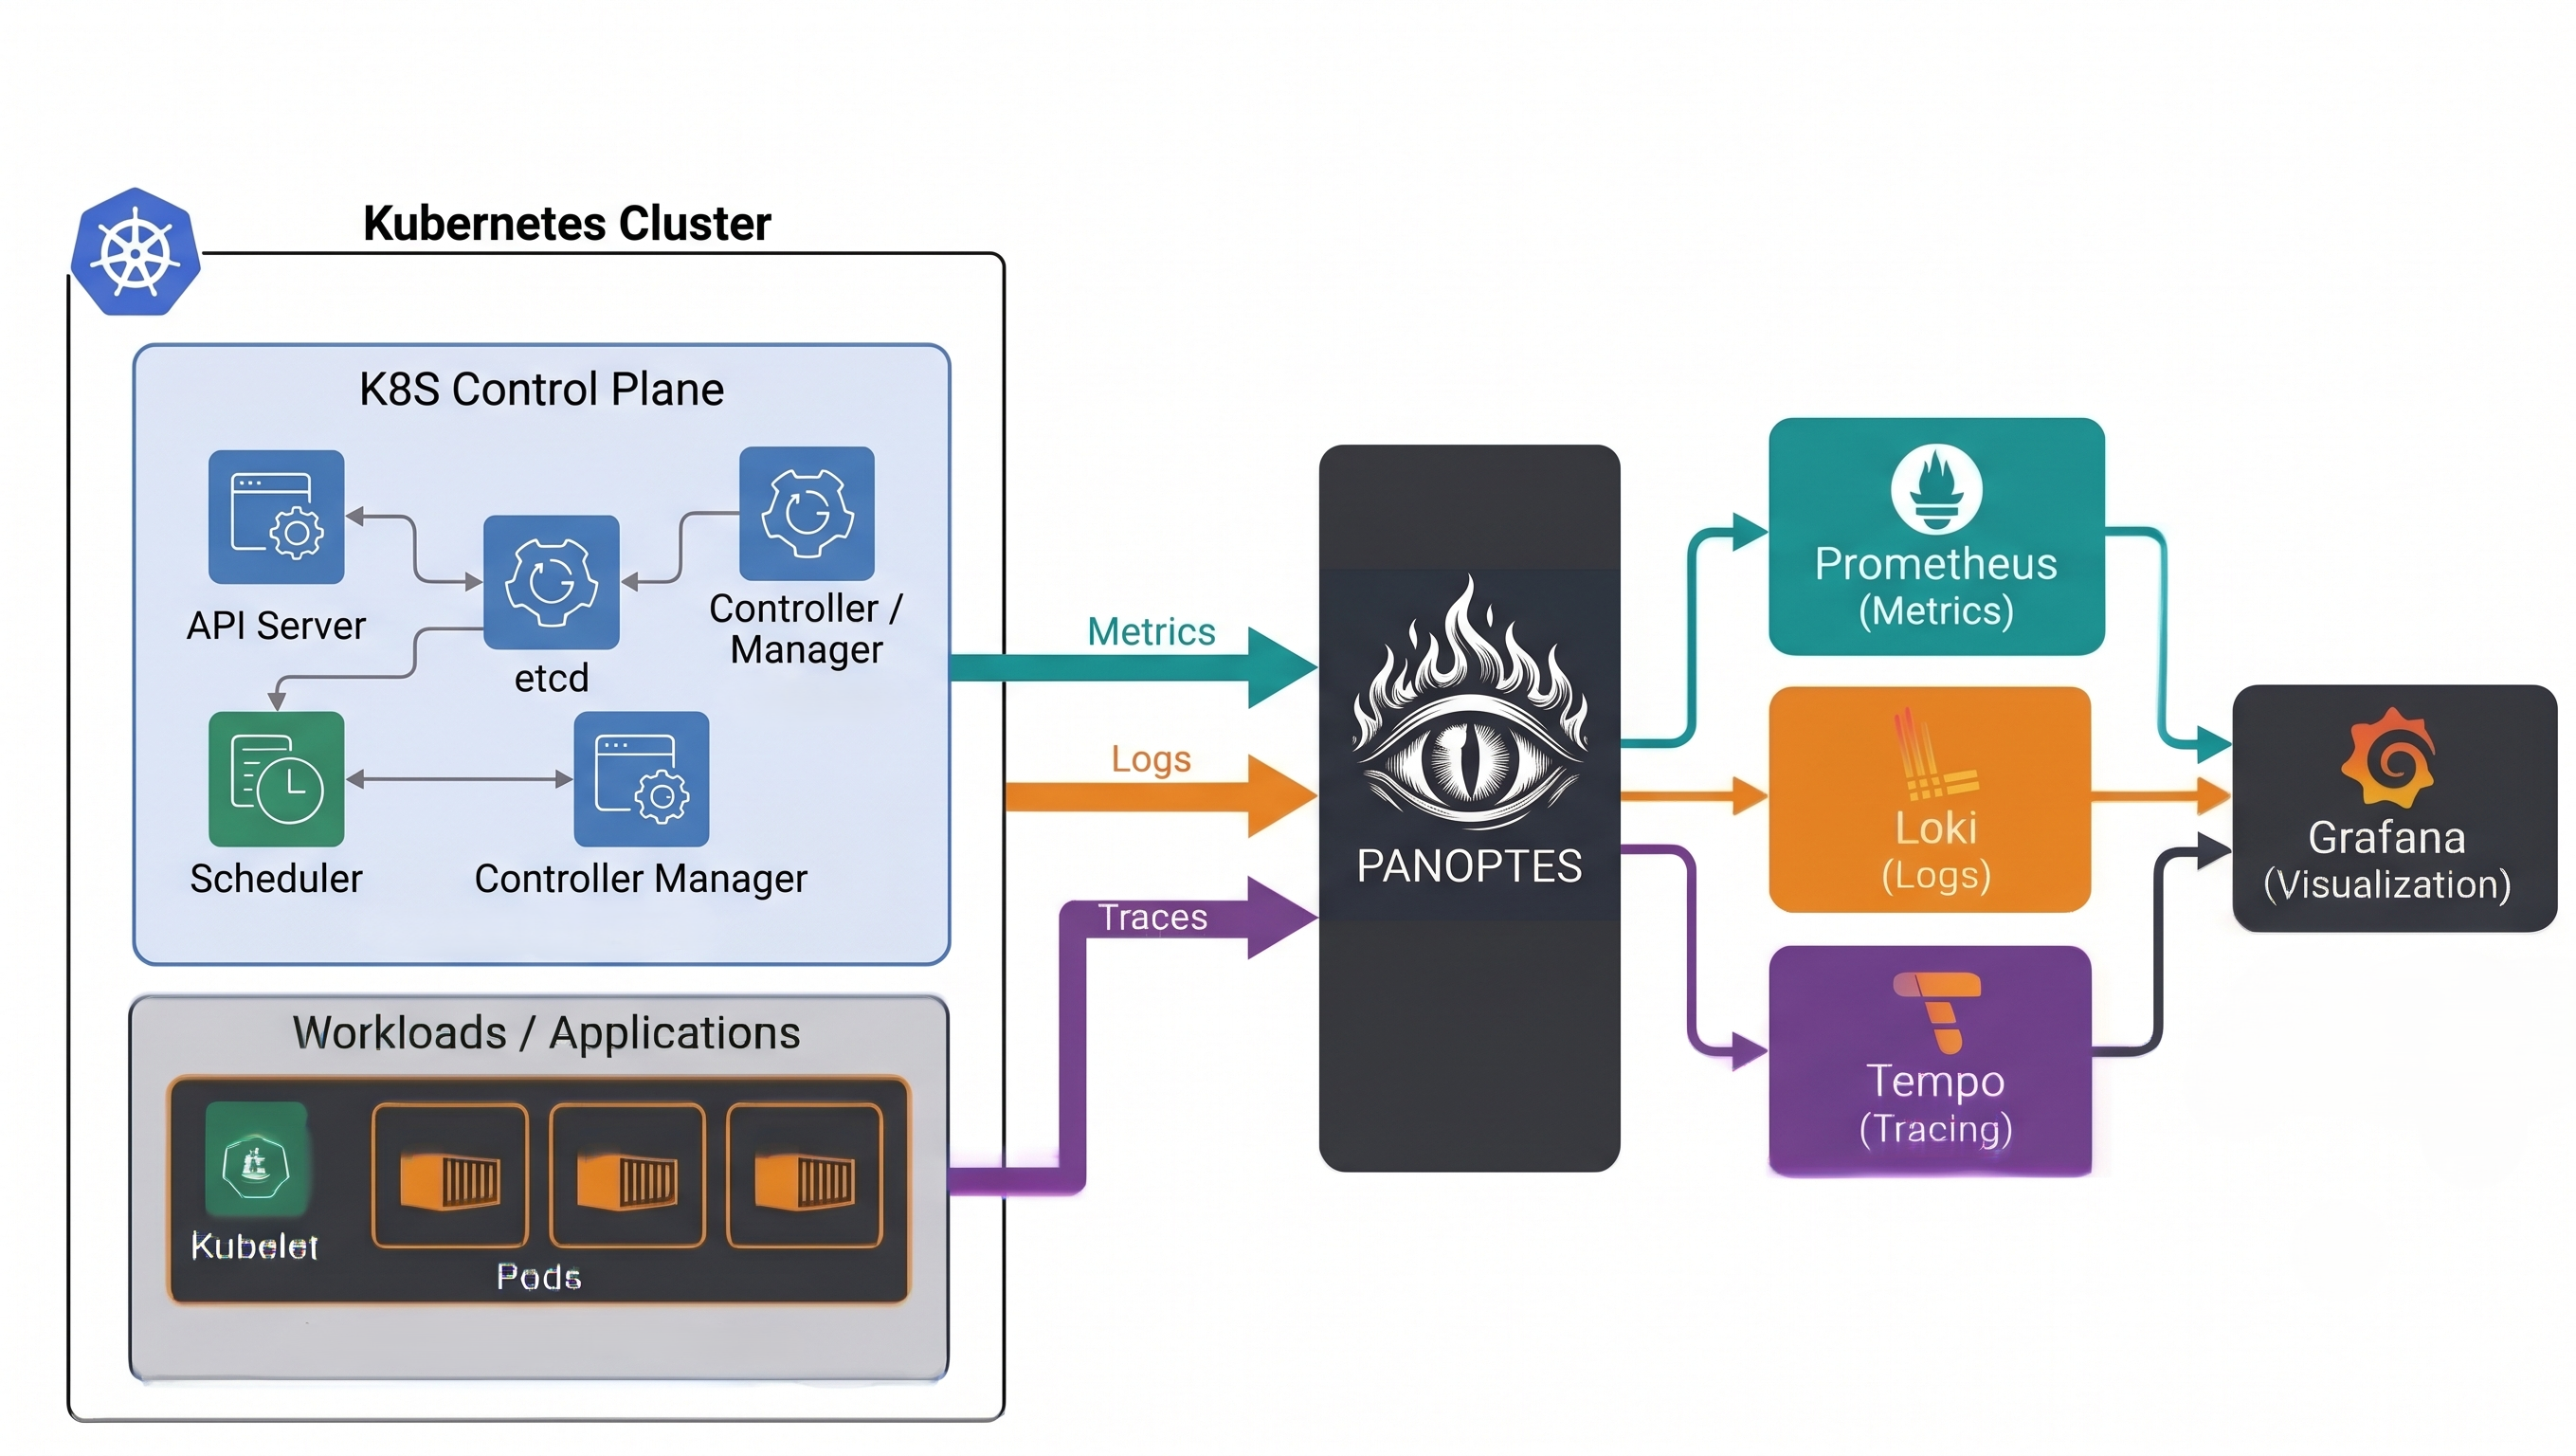
\includegraphics[width=1.0\textwidth]{images/experiment/panoptes_architecture.png}
  \caption{The PANOPTES Reference Architecture for Kubernetes Observability.}
  \label{fig:panoptes_arch}
\end{figure}

As illustrated in Figure \ref{fig:panoptes_arch}, the architecture is systematically divided into three main layers: Signal Generation (OTel), Storage Backends, and the Visualization Layer.

\section{Experimental Environment}
\label{sec:experimental-environment}

The experiments were conducted in a controlled laboratory environment designed to simulate a private cloud infrastructure. To mitigate the ``it works on my machine'' phenomenon and ensure that resource constraints (CPU/RAM) are strictly equal across all scenarios, we utilized Vagrant as the virtualization orchestrator.

While enterprise production environments typically require a High Availability (HA) control plane with at least three master nodes \cite{brendan_tracey_2018} to ensure etcd quorum and fault tolerance, such a topology introduces inherent network and CPU overhead due to state replication. Since the primary objective of this controlled experiment is to evaluate the specific resource overhead ($H_{1b}$) and diagnostic efficiency ($H_{1a}$) of the PANOPTES observability architecture, we adopted a Minimum Distributed Topology consisting of 1 Control Plane (Master) and 2 Worker nodes.

This 3-node configuration is widely adopted in cloud computing experimental research as it achieves two fundamental goals: (1) it strictly isolates the Control Plane components from the Data Plane, ensuring that the measured overhead on the workers is exclusively attributed to the application and the observability agents; and (2) the presence of multiple worker nodes forces inter-node communication, providing a valid and realistic scenario to evaluate Distributed Tracing and network telemetry, which cannot be accurately simulated in single-node environments like Minikube.

\subsection{Virtualization Layer (Vagrant)}
The infrastructure consists of a Kubernetes cluster with one Control Plane node and two Worker Nodes. The specifications for each Virtual Machine (VM) are defined in a \texttt{Vagrantfile}, ensuring that both the Baseline and Experimental groups operate under identical hardware constraints. The vagrant files are declared in appendix \ref{app:vagrant-scripts}.

\begin{table}[h]
\centering
\caption{Virtual Machine Specifications (Per Node)}
\label{tab:vm-specs}
\begin{tabularx}{\textwidth}{|l|l|X|}
\hline
\textbf{Resource} & \textbf{Specification} & \textbf{Justification} \\ \hline
Hypervisor & Multipass (Hyper-V/WSL2) & Canonical's native light-weight VM orchestrator. \\ \hline
OS & Ubuntu Server 22.04 LTS & Standard Linux kernel (5.15) with eBPF support. \\ \hline
vCPU & 2 Cores & Minimum for Kubernetes functional stability. \\ \hline
RAM & 4096 MiB & Sufficient for K8s + Observability Stack + Workload. \\ \hline
Network & Private Bridge & Isolated network to prevent external latency interference. \\ \hline
\end{tabularx}
\par\medskip\ABNTEXfontereduzida\selectfont\textbf{Source:} The author \par\medskip
\end{table}

\subsection{Host Environment Specification}
\label{subsec:host-environment}

To ensure the transparency, internal validity, and full reproducibility of the controlled experiment, it is imperative to detail the hardware and software specifications of the host machine where the virtualized testbeds were executed. The experiment was purposely conducted on a single physical machine to isolate the evaluation environment from external network latencies and multi-tenancy interference (the ``noisy neighbor'' effect) that are typical of public cloud providers.

The baseline and the PANOPTES architecture scenarios were sequentially provisioned on a host machine equipped with an 11th Gen Intel\textsuperscript{\tiny\textregistered} Core\textsuperscript{\tiny\texttrademark} i7-11800H processor (8 Cores, 16 Logical Threads) running at a base frequency of 2.30 GHz, and 64.0 GB of physical RAM. Storage operations were backed by a 1 TB NVMe SSD (SK Hynix PC711). Benchmark evaluations for this specific drive indicate high-performance capabilities, delivering sequential read speeds of 3,021 MB/s and sequential write speeds of 2,461 MB/s. The use of this NVMe protocol is methodologically relevant as it guarantees high Input/Output Operations Per Second (IOPS) and low fsync latency, ensuring the stability of the Kubernetes etcd distributed key-value store without bottlenecking the telemetry collection or generating false-positive overhead readings.

The underlying operating system running on the host is Microsoft Windows 11 Home Single Language (Build 26200). To manage the virtualization layer and provide strict hardware boundaries for the experiment, a Type-2 hypervisor (version 7.2.6) was utilized, fully orchestrated by Vagrant. This setup ensured that both scenarios (Vanilla and PANOPTES) had identical hardware quotas strictly allocated (e.g., specific vCPUs and RAM assigned per node) during their respective execution windows.

To ensure strict reproducibility and mitigate compatibility issues with the observability agents during the Helm deployment phase, the Kubernetes control plane and worker nodes were deterministically locked to version v1.34.5+k3s1 across all experimental scenarios.

Although traditional deployment tools like \textit{kubeadm} are standard for bare-metal production environments, this research adopts Rancher K3s (v1.34.5+k3s1) as the Kubernetes distribution for the experimental testbeds. K3s is a CNCF-certified, lightweight Kubernetes distribution packaged as a single binary. Its use is methodologically justified by its minimal resource footprint, which prevents control-plane starvation in virtualized laboratory environments. By reducing the inherent orchestration overhead, K3s ensures that the baseline resource consumption ($R_{base}$) remains deterministic, isolating the performance metrics exclusively to the target microservices and the evaluated PANOPTES observability architecture.

\input{chapters/06.experiment/sections/03.iac-strategy}

\input{chapters/06.experiment/sections/04.panoptes-instantiation}

\input{chapters/06.experiment/sections/05.target-workload}

\section{Fault Injection Implementation}
\label{sec:fault-injection-impl}

Consistent with the Chaos Engineering methodology defined in Chapter \ref{chap:cloud-computing}, we utilize Chaos Mesh to programmatically inject faults into our target microservices cluster. The experiments defined in Chapter \ref{chap:methodology} are implemented as Kubernetes Custom Resource Definitions (CRDs). To evaluate the diagnostic capabilities of our observability architecture against a wide spectrum of system failures, we implement three declarative fault injection profiles:

\subsection{Pod-Level Disruption (PodChaos)}
The first campaign simulates a hard hardware or runtime crash of a specific service container, forcing Kubernetes to perform self-healing and redeploy the pod. This profile tests the preservation of forensic container logs in Loki after the container is destroyed. The declarative ``Pod Failure'' scenario is codified in Listing \ref{code:pod-chaos}.

\begin{lstlisting}[language=Yaml, caption={Pod Chaos Manifest}, label={code:pod-chaos}]
apiVersion: chaos-mesh.org/v1alpha1
kind: PodChaos
metadata:
  name: frontend-failure
spec:
  action: pod-kill
  mode: one
  selector:
    namespaces:
      - default
    labelSelectors:
      "app": "frontend"
  duration: "60s"
\end{lstlisting}

\subsection{Network-Level Performance Degradation (NetworkChaos)}
The second campaign introduces high-cardinality performance anomalies, injecting synthetic delay on service-to-service communication paths. This tests the semantic linkage of distributed traces in Tempo and metric-level anomalies under cascading latency. The ``Network Latency'' manifest targeting the payment service is codified in Listing \ref{code:network-chaos}.

\begin{lstlisting}[language=Yaml, caption={Network Latency Chaos Manifest}, label={code:network-chaos}]
apiVersion: chaos-mesh.org/v1alpha1
kind: NetworkChaos
metadata:
  name: payment-delay
spec:
  action: delay
  mode: one
  selector:
    namespaces:
      - default
    labelSelectors:
      "app": "payment"
  delay:
    latency: "250ms"
    jitter: "50ms"
    correlation: "25"
  direction: to
  duration: "120s"
\end{lstlisting}

\subsection{Resource Saturation (StressChaos)}
The final campaign simulates resource starvation and operational overload, consuming computational CPU or virtual memory within container limits to assess metric alerts and Prometheus threshold violations. The ``CPU Stress'' manifest designed to saturate the shopping cart microservice is codified in Listing \ref{code:stress-chaos}.

\begin{lstlisting}[language=Yaml, caption={CPU Stress Chaos Manifest}, label={code:stress-chaos}]
apiVersion: chaos-mesh.org/v1alpha1
kind: StressChaos
metadata:
  name: cart-cpu-stress
spec:
  mode: one
  selector:
    namespaces:
      - default
    labelSelectors:
      "app": "cart"
  stressors:
    cpu:
      workers: 2
      load: 100
  duration: "180s"
\end{lstlisting}

This declarative multi-profile approach ensures that the ``stress'' state is deterministic, reproducible, and mathematically identical for both the Vanilla and PANOPTES scenarios.

\section{Experiment Execution Procedure}
\label{sec:execution-procedure}

To ensure statistical reliability and eliminate operator and learning biases, the experimental execution follows a strictly automated and repeatable protocol across all 30 iterations ($N=30$) per scenario \cite{wohlin_2012}. Rather than relying on human operators navigating terminal prompts or graphical interfaces, both the baseline (Scenario~3) and experimental (Scenario~4) diagnostic workflows are executed autonomously by a deterministic Root Cause Analysis (RCA) engine \cite{wang_2024, barata_2026}. The execution procedure follows four sequential phases:

\begin{enumerate}
    \item \textbf{State Restoration and Warm-up:} Prior to each iteration, the cluster environment is restored to a validated, healthy baseline. The orchestrator removes any previously injected chaos resources and issues a \texttt{kubectl rollout status} check across the microservices namespace to confirm that all pods are 100\% available and healthy. A mandatory 20-second cooldown period is enforced to purge pending TCP connections, clear transient kernel queues, and stabilize CPU, memory, and network I/O to steady-state levels \cite{jain_1991, georges_2007}.
    
    \item \textbf{Load Generation:} The polyglot Astronomy Shop workload operates under steady-state traffic driven by its native \textit{loadgenerator} microservice. Synthetic user sessions actively traverse the inter-service graph (e.g., product catalog queries, cart mutations, and checkout sequences) prior to perturbation.
    
    \item \textbf{Blind Fault Injection ($T_0$):} Faults are injected programmatically via Chaos Mesh by applying a calibrated network delay ($2000\,\text{ms} \pm 100\,\text{ms}$) to target pods. To ensure experimental neutrality, a blind randomized injector selects the target microservice at runtime from the critical transaction path ($\text{Pool} = \{\texttt{payment}, \texttt{cart}, \texttt{shipping}, \texttt{currency}\}$). The exact RFC3339 timestamp of the Kubernetes API Server submission is recorded as the authoritative injection start time ($T_0$).
    
    \item \textbf{Algorithmic Diagnosis and Latency Extraction ($T_{\text{diag}}$):} Upon fault activation and an initial 10-second propagation window, the automated diagnostic engine initiates periodic polling (every $5\,\text{s}$) to isolate the injected root cause:
    \begin{itemize}
        \item \textbf{Vanilla Kubernetes (Scenario~3):} The engine interacts exclusively with native Kubernetes CLI endpoints, executing breadth-first log scraping constrained by temporal \texttt{--since-time} filters, regex exception matching, and periodic resource polling via the \texttt{metrics-server} API \cite{wang_2024}.
        \item \textbf{PANOPTES Architecture (Scenario~4):} The engine queries the unified telemetry backends, sampling upper percentile latencies ($p95/p99$) via Prometheus HTTP endpoints, querying Tempo for traces exhibiting anomalous duration, and traversing the call graph to isolate the root span \cite{barata_2026}.
    \end{itemize}
\end{enumerate}

The Mean Time to Diagnose ($MTTDiag$) for each iteration is recorded as the wall-clock execution latency between fault injection and algorithmic convergence:
\begin{equation}
    MTTDiag = T_{\text{diag}} - T_0
\end{equation}
If the diagnostic engine fails to converge on the ground-truth component or exceeds the operational ceiling of $300\,\text{s}$ ($5\,\text{min}$), the iteration is right-censored at $300\,\text{s}$ and flagged as an investigative failure ($Acc = 0$, $\text{censored} = \text{True}$).

\subsection{Automated Orchestration Lifecycle}
\label{subsec:automated-orchestration-lifecycle}

To guarantee experimental replicability and eliminate operator fatigue, observer bias, and clock desynchronization, the complete lifecycle across both experimental groups is governed by out-of-band automation scripts (\texttt{run-scenario3-trials.py} and \texttt{run-scenario4-trials.py}).

The orchestration pipeline executes an automated state machine for each experimental trial:
\begin{enumerate}
    \item \textbf{Cluster State Synchronization:} The orchestrator queries the Kubernetes API to guarantee that all microservices deployments have fully recovered from the preceding trial (\texttt{kubectl rollout status}), followed by the 20-second quiet period to purge transient network buffers and conntrack table entries.
    
    \item \textbf{Dynamic Fault Manifest Generation:} The orchestrator dynamically synthesizes and applies the Chaos Mesh manifest (\texttt{NetworkChaos}) targeting the blindly selected microservice and captures the RFC3339 timestamp ($T_0$).
    
    \item \textbf{Temporal Isolation and Active Polling:} Following a 10-second delay to allow traffic propagation, the RCA engine initiates polling. In the Vanilla baseline, queries to container logs enforce a strict temporal boundary (\texttt{--since-time=}$T_0$), preventing cross-trial contamination from historical log entries.

    \item \textbf{Ground-Truth Convergence and Data Persistence:} When the engine emits its diagnostic verdict, the timestamp is captured as $T_{\text{diag}}$, computing $MTTDiag$. If the diagnosed component matches the ground truth, accuracy is recorded as $Acc = 1$; otherwise, or upon reaching the 300-second ceiling, it is recorded as $Acc = 0$. The trial tuple ($\text{trial\_id}$, $\text{ground\_truth}$, $\text{diagnosed\_target}$, $T_0$, $MTTDiag$, $Acc$, $\text{censored}$) is written to persistent storage, and the chaos manifest is removed.
\end{enumerate}

\subsection{Testbed Commissioning and Telemetry Validation}
\label{subsec:testbed-commissioning}

Prior to the execution of the full $N=30$ trial batteries across the experimental groups, the testbed underwent systematic commissioning and functional validation. This stage verified that the deployment manifests, container runtimes, telemetry pipelines, and fault-injection hooks interact as specified in the architectural design.

\begin{figure}[htbp]
  \centering
  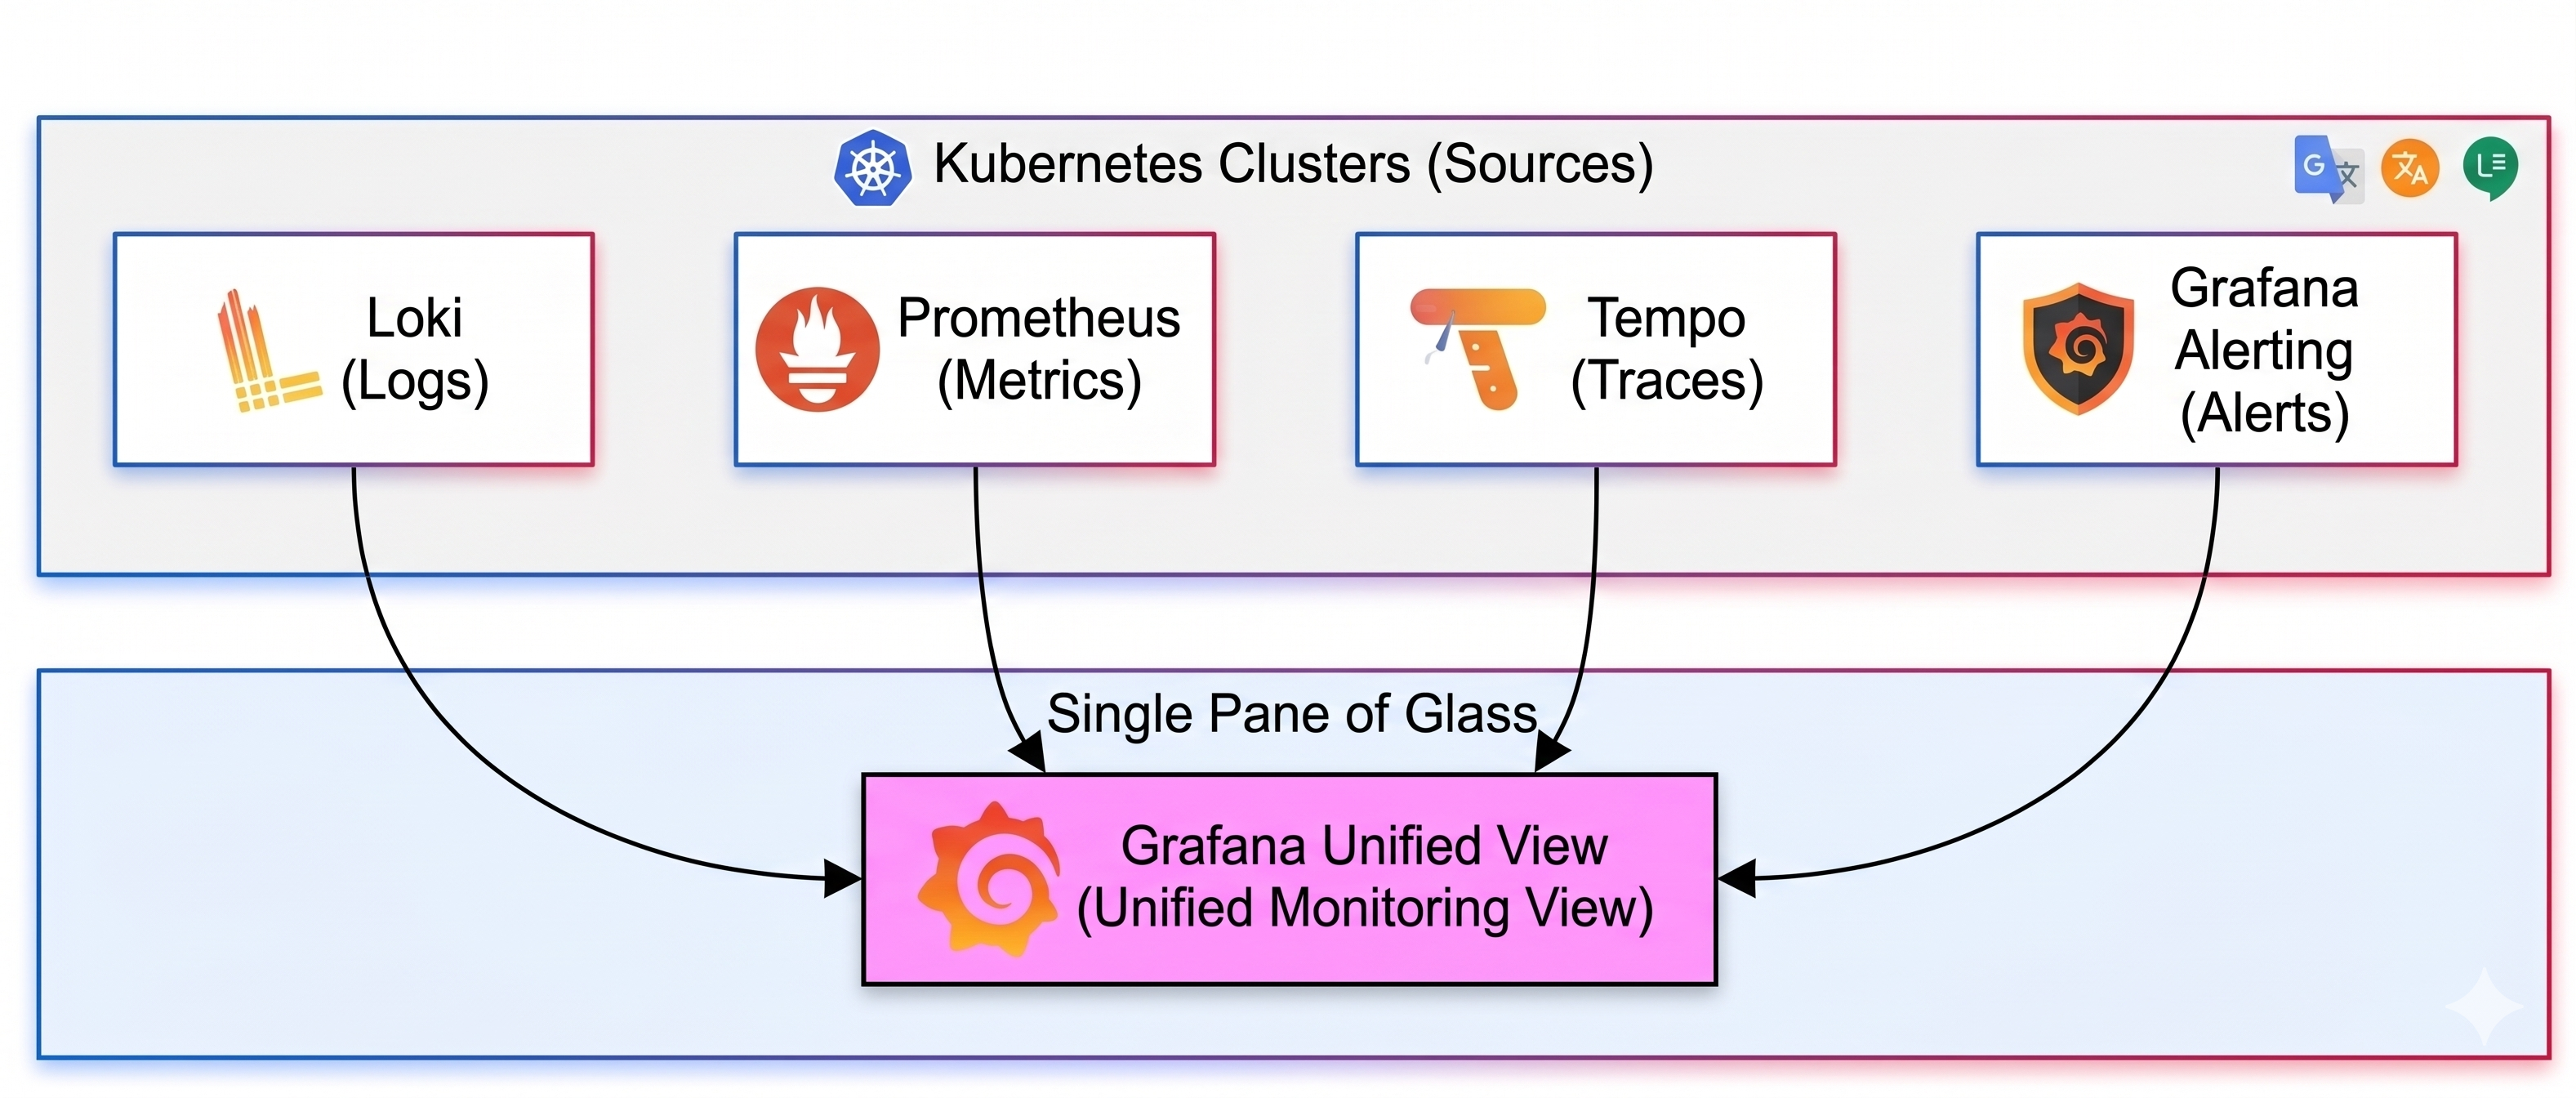
\includegraphics[width=0.9\textwidth]{images/experiment/grafana_preliminary.png}
  \caption{Single Pane of Glass dashboard validating unified telemetry ingestion in Grafana.}
  \label{fig:grafana_preliminary}
\end{figure}

Figure~\ref{fig:grafana_preliminary} demonstrates the operational ``Single Pane of Glass'' dashboard during steady-state workload execution. It validates that the OpenTelemetry collectors actively extract spans, runtime metrics, and container logs from the polyglot microservices, successfully streaming them to their respective storage backends: Prometheus, Grafana Loki, and Grafana Tempo. Furthermore, controlled perturbation trials confirmed that Chaos Mesh successfully manipulates the network namespaces of the target pods (applying netem delays) without destabilizing the underlying K3s control plane, establishing the safety and repeatability of the fault injection mechanism.

While the empirical evaluation of diagnostic latency ($MTTDiag$) is conducted autonomously via programmatic APIs to eliminate human operator bias, Grafana serves as the operational supervisory layer. It validates the underlying semantic binding implemented across the datasource configurations:
\begin{itemize}
    \item \textbf{Metrics to Traces via Exemplars:} The Prometheus datasource binds OpenTelemetry \texttt{traceID} values to latency histograms as exemplars. When an anomalous duration is recorded in the upper latency percentiles ($p95/p99$), the associated exemplar exposes the exact \texttt{traceID}, enabling immediate transition to the corresponding trace graph in Grafana Tempo without manual cross-system lookup.
    
    \item \textbf{Traces to Logs via Contextual Bindings:} The Tempo datasource integrates an automated \textit{Trace to Logs} mapping. For any anomalous span identified within a degraded execution path, the engine synthesizes a LogQL query for Loki. By scoping the search to the specific span timeframe, container namespace, and \texttt{traceID}, it bridges the gap between detecting inter-service latency inflation and inspecting the underlying execution context.
\end{itemize}

These integrated correlation pathways provide interactive root cause navigation within the Grafana interface for post-mortem analysis, while the deterministic RCA engine in Scenario~4 navigates this exact semantic topology programmatically via HTTP endpoints.